\begin{chapter}{Une nouvelle approche d'identification et de dissimulation, de
la détérioration visuelle}
\label{chap-mcb}
Les chapitres antérieurs constituent les éléments d'un panorama technologique
permettant l'assimilation des notions présentées dans ce chapitre. Ces éléments
recouvrent un large territoire technologique s'étendant de l'encodage vidéo à
son transport ainsi que l'impact, la détection et la dissimulation de la
détérioration de séquences vidéos codées en respectant la norme H.264.

Nous rappelons d'abord, à la \sect{sect-limitations}, les limitations des
approches actuelles de détection d'erreurs. Nous présentons ensuite, à la
\sect{sect-MCB}, une amélioration fondamentale aux approches actuelles de
détection de la dégradation visuelle à l'intérieur de trames corrompues. Cette
approche de détection améliorée sert de base pour un nouveau type d'approche de
dissimulation: les approches sélectives. À la \sect{sect-Selectives}, deux
variantes de ces dernières sont décrites.

\begin{section}{Les limitations des approches actuelles de détection de la
détérioration visuelle}
\label{sect-limitations}
Les approches de détection de la détérioration visuelle étudiées ici sont celles
présentées dans notre revue de la littérature. Avant de définir les limitations
de ces approches, commençons par uniformiser la nomenclature utilisée pour les
décrire. Pour ce faire, nous présentons la \fig{fig-System}, soit un survol des
concepts liés à la détection de la détérioration visuelle.

\begin{figure}
	\fbox{
		\includegraphics[width=0.97\linewidth]{images/System.pdf}
	}
	\caption[Survol des concepts liés à la détection de la détérioration
visuelle]{Survol des concepts liés à la détection de la détérioration
visuelle.}
	\label{fig-System}
\end{figure}

Tout d'abord, nous représentons les trames comme des matrices bidimensionnelles
de pixels. Cela dit, $\ltF{}(t)$ fait référence à la $t^{\text{ième}}$ trame
d'une séquence vidéo. Cependant, pour alléger la notation, quand le contexte est
clair, nous n'utilisons pas l'indice de la trame. Par exemple, $\ltF{}(t)$
devient $\ltF{}$. L'image de référence, celle non compressée, est définie par
$\ltF{O}(t)$. De plus, on note $\ltP{}$, la trame qui précède la trame $\ltF{}$,
ce qui équivaut à $\ltF{}(t-1)$.

Pour la transmission sur le canal, une trame est divisée en paquets. Cet
empaquetage est représenté par $p_i(\ltF{})$, où $i$ est l'indice du paquet
associé à la trame $\ltF{}$. Nous désignons la corruption du paquet
$p_i(\ltF{})$ par $\hat{p}_i(\ltF{})$. La trame issue du décodage des paquets
corrompus $\hat{p}_i(\ltF{})$, lorsqu'il est possible, est représentée
par $\ltE{}(t)$, ce qui équivaut à $\hat{\ltF{}}(t)$.

Les auteurs, \citet{Superiori2007} ainsi que \citet{Ikuno2007}, présentent une
approche de détection où l'on mesure l'énergie des blocs ainsi que leurs effets
de blocs à l'intérieur d'un différentiel $\ltD{}$. Ce différentiel, issu de la
différence absolue entre la trame erronée $\ltE{}$ et la trame qui la précède
$\ltP{}$, est défini par la formule suivante~:
\begin{equation}
\ltD{} = \left| \ltE{} - \ltP{} \right|.
\end{equation}
Les données obtenues par ces mesures sont comparées à des seuils et un système
de votes détermine s'il y a erreur. La méthode se base sur l'hypothèse que les
pixels ne varient pas beaucoup d'une image à l'autre et que les grandes
variations sont probablement dues à des erreurs de transmission. Nous
présentons, à titre d'exemple de cette approche, la \fig{fig-FrameDiff} tirée de
\citet[p.~25]{Ikuno2007}. Pour éviter le recours aux seuils, les auteurs
\citet{Farrugia2008} collectent une série de mesures provenant de $\ltD{}$ et
utilisent une machine à vecteurs de support \citep{SVM1995} pour identifier les
blocs erronés.

\begin{figure}
	\fbox{\centering
		\minibox[c]{
			\subfloat[La trame endommagée $\ltE{}$]{
				\includegraphics[width=0.30\linewidth]{images/IkunoBroken.png}
				\label{fig-IkunoBroken}}
			\subfloat[La trame précédente $\ltP{}$]{
				\includegraphics[width=0.30\linewidth]{images/IkunoPrev.png}
				\label{fig-IkunoPrev}}
			\subfloat[Le différentiel $\ltD{}$]{
				\includegraphics[width=0.30\linewidth]{images/FrameDifference.png}
				\label{fig-Diff}}\\
			\subfloat[Analyse du différentiel]{
				\includegraphics[width=0.42\linewidth]{images/FrameDifferenceAnalysis.png}
				\label{fig-DiffAnalysis}}
			\subfloat[Erreurs détectées]{
				\includegraphics[width=0.42\linewidth]{images/FrameDifferenceDetection.png}
				\label{fig-DiffDetection}}
		}
	}
	\caption[Exemple de l'analyse et de la détection d'erreurs]{Exemple de
l'analyse et de la détection d'erreurs. \\Tirée de \citet[p.~25]{Ikuno2007}}
	\label{fig-FrameDiff}
\end{figure}

Le problème commun que nous identifions, comme limitation majeure, avec ces
approches est l'usage du différentiel $\ltD{}$. Quoiqu'il puisse sembler
alléchant, ce dernier, illustré à la \fig{fig-Diff}, ne contient pas uniquement
l'erreur due aux erreurs de transmission, mais aussi la variation des valeurs de
pixels propre à la séquence. Cela signifie que le différentiel résultant des
transformations entre les images non erronées, entre $\ltF{}$ et $\ltP{}$, tel
le mouvement des objets, est aussi contenu dans $\ltD{}$. En effet, utilisant
l'inégalité du triangle ( $\left|a-b\right| \le\left|a-c\right| +
\left|c-b\right| $), on peut réécrire l'équation précédente comme:
\begin{equation}
\ltD{}= \left|\ltE{}-\ltP{}\right| \le   \underbrace{
\left|\ltE{}-\ltF{}\right|}_{\ltD{e}} +   \underbrace{
\left|\ltF{}-\ltP{}\right|}_{\ltD{v}}\:,
\end{equation}
avec $\ltD{e}$ l'erreur produite par les détériorations visuelles dues aux
erreurs de transmission et $\ltD{v}$ l'erreur produite par les variations entre
les trames.  On peut remarquer que sans $\ltF{}$, il est impossible de
distinguer, à l'intérieur de $\ltD{}$, les contributions individuelles de
$\ltD{e}$ et de $\ltD{v}$. Les auteurs mentionnés précédemment
(\citet{Superiori2007}, \citet{Ikuno2007} ainsi que \citet{Farrugia2008}) misent
sur les caractéristiques spatiales de la dégradation visuelle pour tenter
d'effectuer cette distinction. Cependant, il est probable que la variation entre
les trames $\ltD{v}$ manifeste ce genre de caractéristiques. Comme nous le
démontrons aux figures~\ref{fig-CoastDiffGood} et \ref{fig-CoastDiffBad}.

\begin{figure}
	\fbox{\centering
		\minibox{
			\subfloat[$\ltE{}$]{
				\includegraphics[width=0.47\linewidth]{images/coastguardBad.png}
				\label{fig-CoastBad}}
			\subfloat[$\ltD{v}$]{
				\includegraphics[width=0.47\linewidth]{images/coastguardDiffGood.png}
				\label{fig-CoastDiffGood}}\\ %
			\subfloat[$\ltD{}$]{
				\includegraphics[width=0.47\linewidth]{images/coastguardDiffBad.png}
				\label{fig-CoastDiffBad}}
			\subfloat[$\ltD{e}$]{
				\includegraphics[width=0.47\linewidth]{images/coastguardDiffDiff.png}
				\label{fig-CoastDiffDiff}}
		}
	}
	\caption[Contrexemple de l'usage de $\ltD{}$ pour la détection
d'erreurs]{Contrexemple de l'usage de $\ltD{}$ pour effectuer la détection
d'erreurs. Le contenu du différentiel \ref{fig-CoastDiffBad} provient de la
variation entre la trame \ref{fig-CoastBad} et la trame qui la précède.}
	\label{fig-Coastguard}
\end{figure}

Par notre contrexemple, la \fig{fig-Coastguard}, nous démontrons
l'inefficacité de la détection d'erreurs par $\ltD{}$. La séquence
\textit{coastguard} est caractérisée par un déplacement horizontal de la caméra.
Ce déplacement crée une très grande variation entre deux trames consécutives,
comme illustré à la \fig{fig-CoastDiffGood}. L'erreur à détecter est identifiée
à la \fig{fig-CoastDiffDiff}. Il n'est pas simple d'extraire cette information
de $\ltD{}$ (\fig{fig-CoastDiffBad}) sans connaitre $\ltF{}$.

Bref, ce manque de précision, engendré par la variation \textit{intertrame}
présente dans le différentiel, force les auteurs à employer des systèmes
complexes de votes ou de machines à vecteur de support. À l'opposé, le résultat
de notre effort de recherche est une approche de détection simple qui oeuvre
dans un contexte différent de $\ltD{}$, où la variation entre les trames est
minimisée par la compensation de mouvement.
\FloatBarrier
\end{section}

\begin{section}{Les effets de blocs compensés par le mouvement}
\label{sect-MCB}
Nous venons de présenter la variation entre les trames comme un obstacle majeur
à la détection d'erreurs. En s'intéressant aux origines de cette variation, on
constate qu'elle peut provenir d'une translation, d'une déformation, d'un
changement d'intensité lumineuse ainsi que de l'insertion ou du retrait de
contenu. Pour plus d'information sur la détérioration visuelle référez-vous au
chapitre sur la détérioration visuelle \page{chap-erreur}.

En pratique, l'erreur de transmission agit comme un changement entre les trames
équivalant soit à une déformation ou à une insertion de contenu. Ce qui fait en
sorte que ces types de changements sont les plus difficiles à distinguer de
l'erreur.

Dans le domaine de l'encodage vidéo numérique, la variation entre les trames est
un concept qui a suscité une grande quantité d'efforts de recherche. Comme
présentées dans notre section sur H.264 \page{chap-h264}, les approches de
recherche et de compensation de mouvement sont raffinées, depuis maintenant
plusieurs années, pour modéliser cette variation afin d'augmenter le taux de
compression issue de leur encodage. La formule de la recherche des vecteurs de
mouvement a déjà été décrite à la formule \ref{eq-MotionVectors} de la page
\pageref{eq-MotionVectors}, pour plus d'information veuillez consulter
\citep{Drew2004}.

En ce qui a trait à la détection de la détérioration visuelle, la recherche de
vecteurs de mouvement peut servir à prendre en compte la variation entre les
trames ($\ltD{v}$). En contrepartie, les approches qui reposent sur $\ltD{}$
insinuent que $\ltD{v}$ = 0.

Pour illustrer cette affirmation, nous recourons à la \fig{fig-BlockEnery}.
Celle-ci montre la somme des pixels pour chaque macrobloc de la trame à la
\fig{fig-CoastBad}, pour $\ltD{}$ (\fig{fig-BlockDiff}) et le résiduel
(\fig{fig-BlockResidual}). Le résiduel est le différentiel absolu entre le bloc
à évaluer et son meilleur candidat dans la trame précédente.

La première rangée de blocs de la \fig{fig-BlockDiff} nous permet de constater
que pour plusieurs blocs valides, comme le démontre la \fig{fig-CoastDiffDiff},
le pointage obtenu est supérieur à ceux des blocs corrompus. Ceci implique
qu'une approche qui exploite l'énergie des blocs pour effectuer sa détection
effectuerait de fausses détections.

De plus, le bloc avec le pointage le plus élevé, dans la
\fig{fig-BlockResidual}, est non seulement une erreur, mais l'erreur la plus
dérangeante de la \fig{fig-CoastBad}. L'écart de pointage, par rapport au
prochain bloc, est considérable, soit plus de 2000. Notons que le second bloc au
pointage le plus élevé est lui aussi erroné. Cependant, il est beaucoup moins
dérangeant, ce qui justifie l'écart de 2000.

\begin{figure}
	\fbox{\centering
		\subfloat[Somme des pixels des macroblocs de $\ltD{}$]{
			\label{fig-BlockDiff}
			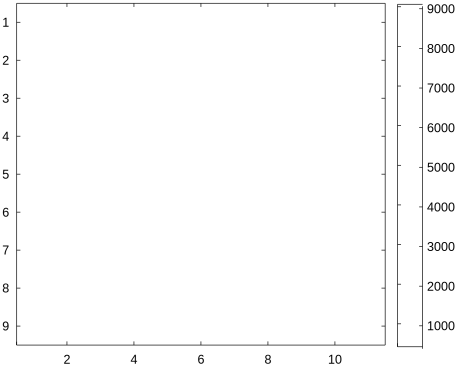
\includegraphics[width=0.47\linewidth]{images/blockDiff.pdf}}
		\subfloat[Somme des pixels des macroblocs du résiduel]{
			\label{fig-BlockResidual}
			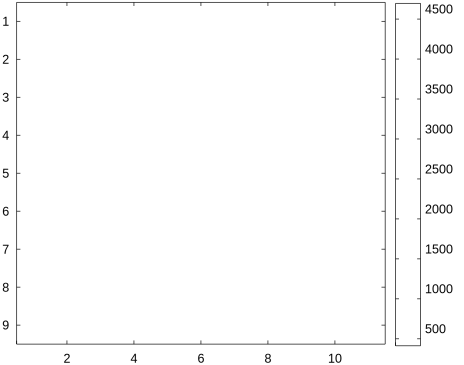
\includegraphics[width=0.47\linewidth]{images/blockResidual.pdf}}
	}
	\caption[Valeurs des macroblocs issues de $\ltD{}$ et du résiduel]{Valeurs des
macroblocs issues de $\ltD{}$~\ref{fig-BlockDiff} et du
résiduel~\ref{fig-BlockResidual} mesurés sur la \fig{fig-CoastBad}.}
	\label{fig-BlockEnery}
\end{figure}

Quoiqu'elle améliore la détection d'erreurs, la compensation de mouvement n'est
pas en mesure d'identifier les vecteurs de mouvement corrompus. Comme décrit au
chapitre \ref{chap-erreur} \page{chap-erreur}, ce type d'erreur insère, dans
l'image erronée, du contenu fautif provenant du mauvais endroit dans la trame de
référence. Pour ce genre d'erreur, la recherche de mouvement retrouve ce contenu
fautif. Ce qui trompe l'algorithme de détection, et ce dernier n'est pas en
mesure d'identifier l'erreur.

Cette limitation de la recherche de mouvement nous oblige à incorporer un
élément important pour la détection d'erreurs: La notion de nuisance. Ce que
nous cherchons à détecter n'est pas l'erreur absolue, mais bien l'erreur qui
engendre une dégradation visuelle perceptible par le système visuel humain. Dans
le chapitre sur l'effet des erreurs sur les séquences vidéos, nous avons conclu
que, pour être dérangeantes, les erreurs doivent exhiber un ou plusieurs effets
de blocs.

\begin{figure}
	\fbox{
		\import{MCB/images/}{MCBExplained.pdf_tex}
	}
	\caption[Visualisation des composantes liées au calcul du MCB]{Visualisation
des composantes liées au calcul du MCB.}
	\label{fig-MCB}
\end{figure}

Les effets de blocs compensés par le mouvement (MCB), que nous proposons dans
cette recherche, sont la combinaison de ces deux faits. Comme décrit à la
\fig{fig-MCB}, le MCB recherche les discontinuités spatiales en bordure de blocs
entre la trame à encoder et la trame de référence. Ne connaissant pas la trame
de référence, nous utilisons la trame précédente.

Avant de procéder à l'explication pratique du fonctionnement du MCB (à la
sous-section \ref{subsect-ExplicationMCB}), nous présentons en détail, à la
section \ref{subsect-theorique}, sa définition mathématique afin de bien
comprendre comment le MCB est mesuré.

\FloatBarrier
\begin{subsection}{Définition théorique du MCB}
\label{subsect-theorique}
Pour cette démonstration, et à des fins de simplicité, nous avons recours à des
blocs carrés\footnoteETS{Il est aussi possible d'utiliser des blocs
rectangulaires.} de taille $B$. Nous définissons un bloc comme un ensemble de
pixels de taille $B\times B$. La hauteur et la largeur d'une trame sont
définies, respectivement, par $H$ et $W$. Les intervalles
$\ltS{m}=[0,\frac{W}{B}-1]$ et $\ltS{n}=[0,\frac{H}{B}-1]$ représentent les
indices de blocs à l'intérieur d'une trame. Nous désignons $p$, comme la
demi-hauteur de la fenêtre de recherche de mouvement.

Nous employons $(u,v)$, comme le vecteur optimal issu de la recherche de
mouvement. Cette opération s'exprime par la formule suivante~: 
\begin{equation}
\label{eq-Vectors}
(\mathbf{U}_{m,n}, \mathbf{V}_{m,n}) = \ltMIN{(u,v) \in K} ~ \ltSAD{mB, nB, u,
v, \ltE{}, \ltP{}} \:,
\end{equation}
où $K = [-p,p] \times [-p, p]$,  $m \in \ltS{m}$, $n \in
\ltS{n}$ et
\begin{equation}
\label{eq-SAD}
\ltSAD{x,y,u,v, \ltE{}, \ltP{}} = \sum_{q=0}^{B-1}\sum_{r=0}^{B-1} \left|
\ltE{x+q,y+r} - \ltP{x+q+u,y+r+v} \right|\:.
\end{equation}
Les composantes des vecteurs de mouvement optimaux $(u,v)$ sont insérées à
l'intérieur des matrices $\mathbf{U}_{}$ et $\mathbf{V}_{}$, à la position
correspondante à l'indice du bloc. Cette opération est effectuée sur l'ensemble
des blocs qui composent la trame $\ltE{}$. Comme il a déjà été mentionné, nous
effectuons la recherche de vecteurs de mouvement afin de tenir compte des
variations issues de $\ltD{v}$ afin de les séparer de la mesure de détérioration
visuelle. Ainsi, au lieu de faire une différence entre les blocs situés à la
même position spatiale, notre métrique effectuera la différence sur les blocs
correspondants d'une trame à l'autre, en considérant leur mouvement. De cette
manière, nous réduisons l'effet du mouvement des objets entre les trames sur la
mesure de différence.

Lors de nos expérimentations, il a été constaté que les gains réalisés par
l'usage d'un niveau de précision au quart et au demi-pixel étaient minimes.
Alors, pour abréger cette démonstration, ces notions ne seront pas présentées
ici. Dans ce chapitre, nous utilisons une précision au pixel entier. Cependant,
nous tenons à informer que des niveaux de précision au quart et au demi-pixel
ont été considérés dans le cadre de nos recherches.

Pour établir l'appariement des blocs entre la trame erronée et la trame de
référence, nous avons recours à la somme de la différence absolue~(SAD) entre
deux blocs~(eq.\ref{eq-SAD}). Quoiqu'il n'en résulte pas une identification
exacte du mouvement, cette approche est peu complexe et permet l'identification
du bloc candidat avec la plus faible variation par rapport au bloc désiré.
Ainsi, lorsque, pour un bloc donné, le SAD minimum est élevé, on peut souvent
conclure qu'une erreur s'est produite.

Toutefois, l'usage du SAD minimum, tel que calculé en (eq.~\ref{eq-Vectors}),
n'est pas efficace comme approche de détection d'erreurs, lorsque le contenu erroné
est présent dans la trame précédente~$\ltP{}$ (c.-à-d. lorsqu'un bloc possède un
bloc similaire dans la trame précédente). Cette situation se présente souvent
lorsque les vecteurs de mouvement sont corrompus. Dans cette situation, ces
vecteurs pointent sur le mauvais contenu même si le SAD est faible, ce qui peut
souvent entrainer des effets de blocs importants.

Comme illustré à la \fig{fig-MCB} \page{fig-MCB}, c'est pour cette raison que
nous mesurons plutôt les effets de blocs en bordure du bloc à évaluer, par rapport aux effets
de blocs du candidat résultant, indiqué par le vecteur $(u,v)$, de la recherche
de mouvement (eq.\ref{eq-Vectors}). Nous nommons ainsi cette opération: mesure
d'effets de bloc compensés par le mouvement. On y réfère aussi par son acronyme
anglais MCB, et elle est définie par la formule~:
\begin{equation}
\label{eq-blk}
\lttBLK{d}{\ltE{},\ltP{}, m,n} = \\ \sum_{l = 0}^{B-1} | \ltCB{d,l}{\ltE{},m B,n
B} - \ltCB{d, l}{\ltP{},m B+\mathbf{U}_{m, n}, n B +\mathbf{V}_{m, n}} |\:,
\end{equation}
où \mbox{$m \in \ltS{m}$}, \mbox{$n \in \ltS{n}$}. De plus, $\mathbf{U}$ et
$\mathbf{V}$ proviennent de l'équation~\eqref{eq-Vectors}. Le MCB est appliqué à
toutes les bordures d'un bloc ($d \in \mathcal{B}$). Nous référons aux bordures
d'un bloc par l'ensemble suivant~: $\mathcal{B}=\{\ltBor{N}, \ltBor{E},
\ltBor{S}, \ltBor{W}\}$ et nous mesurons les vecteurs d'effets de bloc
$\mathbf{b}_{d, l}$ pour chacune d'elles, à l'aide de:
\begin{align}
\ltCB{\ltBor{N}, l}{\ltF{}, x,y} &= \ltF{x+l,y} - \ltF{x+l,y-1}\:, \\
\ltCB{\ltBor{E}, l}{\ltF{}, x,y} &= \ltF{x+B,y+l} - \ltF{x+B-1,y+l}\:, \\
\ltCB{\ltBor{S}, l}{\ltF{}, x,y} &= \ltF{x+l,y+B} - \ltF{x+l,y+B-1}\:, \\
\ltCB{\ltBor{W}, l}{\ltF{}, x,y} &= \ltF{x,y+l} - \ltF{x-1,y+l}\:,
\end{align}
où $l \in [0, B-1]$, et $(x,y)$ sont les
coordonnées en pixels des blocs.

Pour évaluer l'effet global des effets de blocs en bordure d'un bloc, nous
utilisons la somme des effets de blocs compensés par le mouvement de ce dernier
($\textrm{SMCB}$). Cette mesure est obtenue, pour un bloc aux coordonnées de
bloc $(m,n)$, à l'aide de la formule suivante~:
\begin{equation}
\label{eq-SumTB}
\ltSTBLK{\ltF{},\ltP{}, m,n} =
\sum_{d\:\in\:\mathcal{B}}\lttBLK{d}{\ltF{},\ltP{},m,n}\:.
\end{equation}

Dans cette formule, on effectue la sommation des valeurs MCB pour chacune des
bordures $d \in \mathcal{B}$ du bloc évalué. Ce qui est intéressant avec cette
nouvelle approche, c'est que nous mesurons le niveau de discontinuité présent à
la bordure du bloc, obtenue en soustrayant le bloc considéré du bloc qui lui
correspond le mieux dans l'image précédente. S'il n'y a aucun bloc candidat
correspondant bien au bloc considéré ou si le bloc correspond bien, mais qu'il
provient de l'application d'un mauvais vecteur de mouvement et, par conséquent
il est ainsi hors de son contexte initial, la mesure est élevée. Sinon, un objet
s'est seulement déplacé et, par conséquent le contexte visuel est le même autour
du bloc considéré et du bloc candidat, même s'il y a beaucoup de détails ou de
bordures marquées autour de ces blocs, alors la mesure obtenue sera faible par
l'effet soustractif du MCB.

Les figures~\ref{fig-Good},~\ref{fig-Bad1} et~\ref{fig-Bad2} montrent la mesure
des effets de bloc compensés par le mouvement dans trois situations différentes
choisies parmi celles rencontrées lors du décodage de séquence H.264. Pour
chaque situation, les quatre bordures (nord, est, sud, ouest) extérieures du
bloc à évaluer, encadré en rouge dans \ref{fig-ExemplesGood}, sont comparées
à celles du meilleur bloc candidat, de la trame précédente, encadré en rouge
dans \ref{fig-ExemplePrev}.

\begin{figure}
	\fbox{\centering
		\minibox[c]{
			\subfloat[Trame à évaluer]{
				\label{fig-ExemplesGood}
				\includegraphics[width=0.42\linewidth]{images/Exemples_Good.png}}
			\subfloat[Trame précédente]{
				\label{fig-ExemplePrev}
				\includegraphics[width=0.42\linewidth]{images/Exemples_Prev.png}}\\
			\subfloat[\scriptsize Nord]{
				\label{fig-GoodTop}
				\includegraphics[width=0.07\linewidth]{images/GoodBordersTop.pdf}}
			\subfloat[\scriptsize Est]{
				\label{fig-GoodRight}
				\includegraphics[width=0.07\linewidth]{images/GoodBordersRight.pdf}}
			\subfloat[\scriptsize Sud]{
				\label{fig-GoodBottom}
				\includegraphics[width=0.07\linewidth]{images/GoodBordersBottom.pdf}}
			\subfloat[\scriptsize Ouest]{
				\label{fig-GoodLeft}
				\includegraphics[width=0.07\linewidth]{images/GoodBordersLeft.pdf}}
		}
	}
	\caption[Exemple du MCB pour une trame normale] {Exemple de la mesure des effets
de bloc compensés par le mouvement, pour une trame normale.}
	\label{fig-Good}
\end{figure}

Dans la première situation, illustrée à la \fig{fig-Good}, la trame à évaluer ne
contient pas d'erreur. Cependant, on y constate un changement important de
l'emplacement du cercle rouge. Dans une telle situation, le différentiel ne
serait pas efficace. Néanmoins, la translation est prise en compte, grâce à la
recherche de mouvement, ce qui fait que les quatre bordures externes sont
identiques.

\begin{figure}
	\fbox{\centering
		\minibox[c]{
			\subfloat[Trame à évaluer]{
				\label{fig-ExemplesBad1}
				\includegraphics[width=0.42\linewidth]{images/Exemples_Bad1.png}}
			\subfloat[Trame précédente]{
				\label{fig-ExemplesPrevBad1}
				\includegraphics[width=0.42\linewidth]{images/Exemples_PrevBad1.png}}\\
			\subfloat[\scriptsize Nord]{
				\label{fig-Bad1Top}
				\includegraphics[width=0.07\linewidth]{images/Bad1BordersTop.pdf}}
			\subfloat[\scriptsize Est]{
				\label{fig-Bad1Right}
				\includegraphics[width=0.07\linewidth]{images/Bad1BordersRight.pdf}}
			\subfloat[\scriptsize Sud]{
				\label{fig-Bad1Bottom}
				\includegraphics[width=0.07\linewidth]{images/Bad1BordersBottom.pdf}}
			\subfloat[\scriptsize Ouest]{
				\label{fig-Bad1Left}
				\includegraphics[width=0.07\linewidth]{images/Bad1BordersLeft.pdf}}
		}
	}
	\caption[Exemple du MCB pour un macrobloc corrompu]{Exemple de la mesure des
effets de bloc compensés par le mouvement, pour un macrobloc corrompu.}
	\label{fig-Bad1}
\end{figure}

La seconde situation est celle du macrobloc corrompu, comme présenté à la
\fig{fig-Bad1}. Dans un tel contexte, le macrobloc corrompu n'existe pas dans la
trame précédente. Ceci fait en sorte que la recherche de mouvement ne réussira
pas à trouver un bon candidat. Certaines implémentations d'algorithmes de
recherche de vecteurs de mouvement, pour des SAD équivalents, vont favoriser les
vecteurs de mouvement plus petits. Dans la situation présentée à la
\fig{fig-ExemplesBad1}, le candidat présenté par la \fig{fig-ExemplesPrevBad1}
est donc plausible. La comparaison des bordures compensées par le mouvement
indique que trois bordures sont différentes (\ref{fig-Bad1Right},
\ref{fig-Bad1Bottom}, \ref{fig-Bad1Left}), ce qui augmente le pointage du
macrobloc de sorte à en permettre l'identification comme macrobloc erroné.

\begin{figure}
	\fbox{\centering
		\minibox[c]{
			\subfloat[Trame à évaluer]{
				\label{fig-ExemplesBad2}
				\includegraphics[width=0.42\linewidth]{images/Exemples_Bad2.png}}
			\subfloat[Trame précédente]{
				\label{fig-ExemplesPrevBad2}
				\includegraphics[width=0.42\linewidth]{images/Exemples_PrevBad2.png}}\\
			\subfloat[\scriptsize Nord]{
				\label{fig-Bad2Top}
				\includegraphics[width=0.07\linewidth]{images/Bad2BordersTop.pdf}}
			\subfloat[\scriptsize Est]{
				\label{fig-Bad2Right}
				\includegraphics[width=0.07\linewidth]{images/Bad2BordersRight.pdf}}
			\subfloat[\scriptsize Sud]{
				\label{fig-Bad2Bottom}
				\includegraphics[width=0.07\linewidth]{images/Bad2BordersBottom.pdf}}
			\subfloat[\scriptsize Ouest]{
				\label{fig-Bad2Left}
				\includegraphics[width=0.07\linewidth]{images/Bad2BordersLeft.pdf}}
		}
	}
	\caption[Exemple du MCB pour un vecteur de mouvement corrompu]{Exemple de la
mesure des effets de bloc compensés par le mouvement, pour un vecteur de
mouvement corrompu.}
	\label{fig-Bad2}
\end{figure}

Le vecteur de mouvement corrompu est notre troisième et dernière situation.
Celle-ci est illustrée à la \fig{fig-Bad2}. La particularité de cette situation
est que le macrobloc erroné est présent dans la trame précédente et sera
retrouvé par l'algorithme de recherche de vecteur de mouvement. Cependant, la
comparaison des bordures extérieures démontre que les pixels externes ne
s'agencent pas (\ref{fig-Bad2Right},
\ref{fig-Bad2Bottom}, \ref{fig-Bad2Left}). Ceci fait en sorte que nous
sommes en mesure d'identifier ce macrobloc erroné.

La détection d'effets de bloc par la mesure de pixels en bordure de blocs peut
toutefois introduire de fausses détections pour les bordures de blocs avoisinant
un bloc erroné. Comme illustré à la \fig{fig-GridSMCB}, dans une telle
situation, la valeur du SMCB des blocs voisins de la détérioration visuelle est
considérablement augmentée par la bordure limitrophe de l'erreur.

\begin{figure}
	\fbox{\centering
		\subfloat[Valeurs MCB et SMCB]{
			\label{fig-GridSMCB}
			\includegraphics[width=0.40\linewidth]{images/Grid3x3_SMCB.pdf}}
		\subfloat[Valeurs distribuées MCB et SMCB]{
			\label{fig-GridSDMCB}
			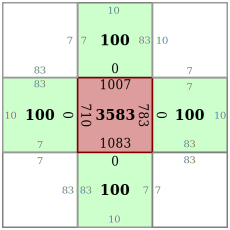
\includegraphics[width=0.40\linewidth]{images/Grid3x3_SDMCB.pdf}}
		\subfloat{
			\label{fig-colorbar}
			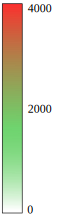
\includegraphics[width=0.11\linewidth]{images/SDMCB_colorbar.pdf}}
	}
	\label{fig-GridMCB}
	\caption[Valeurs MCB et SMCB avant et après la distribution de bordures] {Valeurs MCB des bordures et valeurs SMCB (au centre) des blocs avant
\ref{fig-GridSMCB} et après \ref{fig-GridSDMCB} la distribution de
bordures.}
\end{figure}

Pour résoudre ce problème, nous proposons le SDMCB, soit une version du SMCB où
les bordures à valeurs élevées sont distribuées. La distribution de bordures est
guidée par la valeur du SMCB. La valeur d'une bordure élevée est assignée au
bloc avec le plus grand SMCB. La \fig{fig-GridMCB} montre le résultat de la
distribution et l'algorithme~\ref{algo-SDMCB}~(p.\pageref{algo-SDMCB}) démontre
comment celle-ci est effectuée.


\begin{algorithm}
\caption{Distribution de bordures}
\label{algo-SDMCB}
\algsetup{linenodelimiter=\hspace{2 em}}
\begin{algorithmic}[1]
\STATE \COMMENT{Bordure supérieure}
\IF {$\ltSTBLK{\ltF{},\ltP{}, m,n} < \ltSTBLK{\ltF{},\ltP{}, m,n-1}$} 
\STATE $\lttBLK{\ltBor{N}}{\ltF{},\ltP{}, m,n} = 0$ \ELSE \STATE
$\lttBLK{\ltBor{S}}{\ltF{},\ltP{},m,n-1} = 0$ \ENDIF \STATE \STATE
\COMMENT{Bordure droite}
\IF {$\ltSTBLK{\ltF{},\ltP{},m,n} < \ltSTBLK{\ltF{},\ltP{},m+1,n}$} 
\STATE $\lttBLK{\ltBor{E}}{\ltF{},\ltP{},m,n} = 0$ \ELSE \STATE
$\lttBLK{\ltBor{W}}{\ltF{},\ltP{},m+1,n} = 0$ \ENDIF \STATE \STATE
\COMMENT{Bordure inférieure}
\IF {$\ltSTBLK{\ltF{},\ltP{},m,n} < \ltSTBLK{\ltF{},\ltP{},m,n+1}$} 
\STATE $\lttBLK{\ltBor{S}}{\ltF{},\ltP{},m,n} = 0$ \ELSE \STATE
$\lttBLK{\ltBor{N}}{\ltF{},\ltP{},m,n+1} = 0$ \ENDIF \STATE \STATE
\COMMENT{Bordure gauche}
\IF {$\ltSTBLK{\ltF{},\ltP{},m,n} < \ltSTBLK{\ltF{},\ltP{},m-1,n}$} 
\STATE $\lttBLK{\ltBor{W}}{\ltF{},\ltP{},m,n} = 0$ \ELSE \STATE
$\lttBLK{\ltBor{E}}{\ltF{},\ltP{},m-1,n} = 0$ \ENDIF
\end{algorithmic}
\end{algorithm}
 
Cet algorithme de distribution de bordures, montré à
l'algorithme~\ref{algo-SDMCB} (p.\pageref{algo-SDMCB}), est appliqué, en ordre
décroissant de valeur de SMCB, sur tous les blocs dont la valeur de SMCB est
supérieure à un seuil $T_b$. Le recours au seuil est justifié, car si la valeur
du SMCB est trop basse, la distribution n'est pas précise et ne sert à rien. Le
but de la distribution est d'éviter la propagation des effets de bloc importants
aux blocs voisins. Le seuil $T_b$ établit la valeur à partir de laquelle un bloc
est considéré comme ayant des effets de bloc importants. \FloatBarrier
\end{subsection}

\begin{subsection}{Explication de l'approche MCB}
\label{subsect-ExplicationMCB}

L'approche MCB comporte deux composantes clés pour l'identification d'erreurs.
La première est spatiale, l'analyse de bordures identifie les discontinuités
entre les pixels en bordure de blocs. Toutefois, ces discontinuités pourraient
appartenir à l'image. La seconde composante est temporelle et, dans ce cas,
recherche ces discontinuités dans la trame précédente.

L'insertion ou la déformation de contenu causant un effet de bloc important est
le seul cas problématique. Il est rare et l'effet de bloc doit être
considérablement important pour être considéré comme erroné. Nous présentons à
la \sect{sect-Selectives} notre approche de détection d'erreurs à l'aide des
valeurs de MCB.

\begin{figure}
	\fbox{\centering
		\subfloat[SMCB]{
			\label{fig-BlockSMCB}
			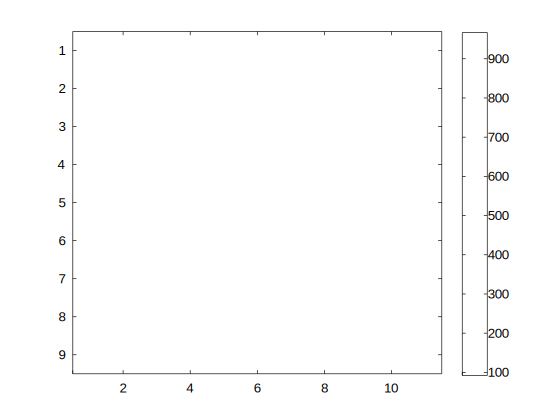
\includegraphics[width=0.47\linewidth]{images/BlockSMCB.pdf}} 
		\subfloat[SDMCB]{
			\label{fig-BlockSDMCB}
			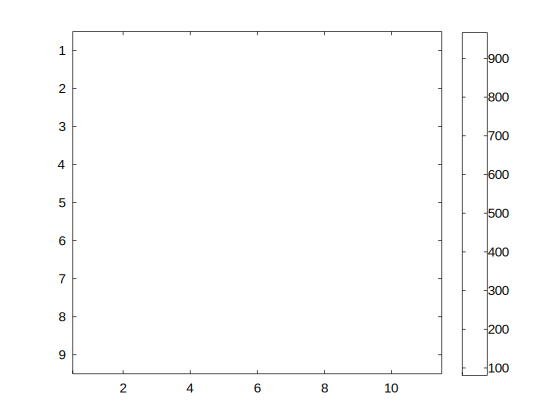
\includegraphics[width=0.47\linewidth]{images/BlockSDMCB.pdf}}
	}
	\caption[Approches de détection d'erreurs basées sur le MCB]{Approches de
détection d'erreurs basées sur le MCB, mesurées par rapport à la
\fig{fig-CoastBad}. Pour l'approche SDMCB, un seuil $T_b=900$ a été utilisé.}
	\label{fig-BlockMCB}
\end{figure}


Nous présentons, à la \fig{fig-BlockMCB}, les résultats obtenus de l'utilisation
des approches SMCB et SDMCB sur la trame erronée de la \fig{fig-CoastBad}
\page{fig-CoastBad}. On y constate en \ref{fig-BlockSDMCB} une réduction
importante des valeurs des blocs, non erronés, voisins aux macroblocs erronés (c.-à-d. $\text{SMCB} >
800$). Rappelons que la propagation d'erreur due à l'usage des bordures
extérieures cause cette augmentation des valeurs des macroblocs non erronés.

En ce qui a trait à la détection d'erreur, nous observons que le SDMCB détecte
l'erreur la plus dérangeante de la \fig{fig-CoastBad} \page{fig-CoastBad}. De
plus, en regardant l'erreur identifiée à la \fig{fig-CoastDiffDiff}
\page{fig-CoastDiffDiff}, nous constatons que les valeurs les plus élevées de
SDMCB (c.-à-d. $\text{SDMCB} > 800$) sont assignées à des macroblocs qui ont
subi une détérioration visuelle. Les valeurs basses de SDMCB (c.-à-d.
$\text{SDMCB} < 200$) sont assigné à des blocs qui ne contiennent pas d'erreurs.
Certes, une zone d'incertitude existe entre 200 et 800, cependant, la
détérioration visuelle contenue par les macroblocs de cette plage de valeurs
n'est pas importante, et les gains de leur dissimulation sont minimes.

À première vue, la comparaison du SDMCB par rapport aux autres approches comme
le résiduel et le différentiel $\ltD{}$ n'est pas évidente. Cependant, en
regardant la zone d'incertitude de $\ltD{}$, soit d'environ 1000 à 9000 (voir
\fig{fig-BlockDiff} \page{fig-BlockDiff}), on constate qu'il n'est pas possible
de distinguer la détérioration visuelle la plus dérangeante $\ltD{e}$ à la
variation entre les trames $\ltD{v}$. \FloatBarrier
\end{subsection}

\end{section}

\begin{section}{Les approches sélectives de dissimulation de la détérioration
visuelle}
\label{sect-Selectives}
Dans cette section, nous sortons du contexte théorique de la détection d'erreurs
et nous offrons une solution pratique de l'application du MCB. Cette solution a
pour but d'améliorer la qualité visuelle des dissimulations effectuées par le
décodeur de référence H.264. Dans le cadre de nos recherches, nous avons intégré
notre solution dans le décodeur du \ltCodec, mais il est aussi concevable de le
voir comme un module d'extension (\textit{plugiciel}) destiné à d'autres
décodeurs.

L'approche MCB assigne une valeur numérique à un bloc évalué en fonction de
l'écart de son effet de bloc par rapport au bloc qui lui ressemble le plus dans
la trame précédente. Nous affirmons, résultats à l'appui\footnoteETS{Voir le
chapitre Résultats et analyse \page{chap-resultats}.}, que cette approche permet
d'identifier les détériorations visuelles importantes dans une trame corrompue.
La quantification de la notion d'une dégradation visuelle importante a été un
problème colossal que nous avons eu à surmonter, lors de notre implémentation
pratique.

Une solution simple est l'usage d'un seuil. Cette valeur numérique définit un
point après lequel un bloc avec un certain SDMCB est considéré comme erroné. Ce
type d'approche, employée par \citet{Superiori2007} ainsi que \citet{Ikuno2007},
ne tient pas compte du caractère variant du contenu d'une séquence vidéo.

L'effet de bloc est relatif à l'image dans laquelle il est perçu. Ceci implique
que l'usage d'un seuil fixe ne sera pas en mesure d'identifier les erreurs dans
des séquences où les caractéristiques spatiotemporelles divergent.

De cette observation est née l'approche sélective. Comme son nom l'identique,
cette approche repose sur la notion d'un choix. Ce changement de paradigme
provient du constat suivant : dans un contexte pratique, la dissimulation est
inutile si l'erreur ne peut être dissimulée. Il est préférable de se concentrer
sur le contenu que nous sommes en mesure de dissimuler.

En nous basant sur le fait que nous cherchons à effectuer une dissimulation,
nous prenons d'un côté une dissimulation traditionnelle, tels la trame calquée
ou le calque des vecteurs de mouvement, et nous la comparons à la trame à
évaluer. Par la suite, nous choisissons la plus petite valeur SDMCB, que ce soit
pour une trame, comme à la section~\ref{sect-SelectiveTrame}, ou pour un
macrobloc, section~\ref{sect-SelectiveBloc}.

Ces approches se comportent comme des seuils dynamiques capables de s'adapter
non seulement au contenu, mais aussi à l'aptitude de dissimulation du macrobloc
évalué. Les approches sélectives effectuent une dissimulation d'un macrobloc,
seulement lorsque du contenu de qualité visuelle supérieure (jugée par le SDMCB)
est disponible.

Une considération pratique importante est le temps de calcul requis par notre
algorithme. Ce temps est restreint, vu les contraintes du \textit{temps réel}
ainsi que les limitations matérielles des appareils mobiles. Ce qui est
dispendieux en terme de temps de calcul pour le MCB est la recherche des
vecteurs de mouvement. Cependant, les récentes avancées dans ce domaine, telles
PMVFAST \citep{Tourapis2001} et UMHexagonS \citep{Cai2009} réduisent de façon
substantielle le temps de calcul requis pour trouver les vecteurs de mouvement.
De plus, notons que dans ce contexte, le décodeur est informé par les entêtes
RTP des paquets corrompus et mesure le SDMCB uniquement pour les trames qui en
résultent.

\begin{subsection}{L'approche sélective au niveau de la trame}
\label{sect-SelectiveTrame}
Notre première approche sélective repose sur le choix d'une trame. Lorsque des
trames sont corrompues, le décodeur peut recourir à plusieurs trames pour la
dissimulation : la tranche calquée, la tranche issue du calque des vecteurs de
mouvement et la trame endommagée. 

Le pointage SDMCB d'une trame est obtenu par la sommation des valeurs du SDMCB
pour chacun de ses macroblocs. Cette sommation est décrite par la formule~:
\begin{equation}
\label{eq-ConcealmentCandidate}
c_c=\sum_{m=0}^{\frac{W}{B}-1}\sum_{n=0}^{\frac{H}{B}-1}\ltSDMCB{\ltConc{}}\:,
\end{equation}
où $\ltConc{}$ est une trame dissimulée par le décodeur, soit une tranche
calquée ou une tranche issue du calque des vecteurs de mouvement, etc. On
mesure une seconde sommation des valeurs SDMCB pour chaque bloc d'une trame.
Cette fois, nous utilisons la trame endommagée $\ltE{}$~:
\begin{equation}
\label{eq-ErroneousCandidate}
c_e=\sum_{m=0}^{\frac{W}{B}-1}\sum_{n=0}^{\frac{H}{B}-1}\ltSDMCB{\ltE{}}\:,
\end{equation}
Par la suite, la trame avec le plus petit pointage est choisie comme
dissimulation $\ltOpt{}$~:
\begin{equation}
\label{eq-SelectiveConcealment}
\ltOpt{} =
\begin{cases}
\ltE{}, & \mathrm{si~} c_e < c_c\\
\ltConc{}, & \mathrm{sinon}
\end{cases}\:.
\end{equation}

\end{subsection}

\begin{subsection}{L'approche sélective au niveau du macrobloc}
\label{sect-SelectiveBloc}
Notre deuxième approche offre un niveau de granularité supérieur à celle de la
première approche, en effectuant la sélection pour chaque macrobloc. Le but de
cette approche est de tirer profit du gain mutuel de différentes approches en
fonction des caractéristiques spatiotemporelles des régions d'images.

Dans certaines conditions, la tranche calquée est optimale; dans d'autres, c'est
la trame erronée ou bien le calque des vecteurs de mouvement. De cette approche
résulte une trame de dissimulation formée d'un conglomérat de macroblocs
optimaux (jugés selon le SDMCB) issus de différents macroblocs candidats pour
la dissimulation.

La dissimulation résultant de la sélection d'un bloc parmi ceux aux indices
$(m,n)$ provenant de la trame corrompue $\ltE{}$ ou de la trame issue de la
dissimulation par calquage de tranches $\ltConc{}$ est obtenue à l'aide de
\begin{equation}
\label{eq-SelectiveConcealment}
\ltOpt{x,y} =
\begin{cases}
\ltE{x,y}, & \mathrm{si~} \ltSDMCB{\ltE{}} < \ltSDMCB{\ltConc{}}\\
\ltConc{x,y}, & \mathrm{sinon}
\end{cases}\:,
\end{equation}
pour tout $x\in mB+[0,B-1]$, tout $y \in nB+[0,B-1]$, et pour tout bloc de
l'image (c.-à-d. $m \in \ltS{m}=[0,\frac{W}{B}-1]$, et $n \in
\ltS{n}=[0,\frac{H}{B}-1]$).
\end{subsection}
\end{section}

Dans ce chapitre, nous avons présenté deux variantes d'un nouveau type
d'algorithme sélectif apte à la dissimulation d'erreurs. Ces variantes agissent
à deux différents niveaux de la hiérarchie de la vidéo numérique, soit ceux des
macroblocs et ceux des trames. Pour guider la sélection, nous proposons un
algorithme de détection d'erreurs fondé sur une nouvelle notion: les effets de
bloc compensés par le mouvement. Cette dernière prend en compte une partie des
changements \textit{intertrame}. Ceux-ci, comme nous avons démontré, entravent
la détection des algorithmes existants.

Le chapitre subséquent porte sur l'analyse des résultats expérimentaux obtenus
à l'aide de notre banc d'essai, conçu pour valider les notions présentées dans
ce chapitre.
\end{chapter}